
\begin{infocard}{Volumen de un cilindro recto}
    \begin{wrapfigure}{r}{0.25\linewidth}
        \centering
        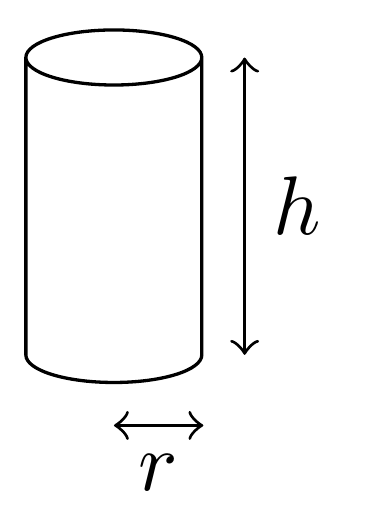
\includegraphics[width=\linewidth]{../images/LpV1W}
    \end{wrapfigure}
    El volumen de un cilindro recto cuya base tiene un área de $A=\pi r^2$, se obtiene mediante la expresión
    \[  V = \pi r^2h  \]
    donde $r$ es el radio del círculo y $h$ la altura del cilindro.
\end{infocard}
